%%% LaTeX Template: Article/Thesis/etc. with colored headings and special fonts
%%%
%%% Source: http://www.howtotex.com/
% vim: set spell spelllang=es syntax=tex :

\documentclass[12pt]{article}
\usepackage{styles/apuntes-estilo}
\usepackage{styles/egyptian}
\usepackage{fancyhdr,lastpage}
\usepackage{hyperref}
\usepackage[inline]{enumitem}

\def\maketitle{

\makeatletter
{\color{bl} \centering \huge \sc \textbf{Recuperatorio del segundo examen
\mbox{parcial}}}
\makeatother

\makeatletter
% vim: set spell spelllang=es syntax=tex :
 {\centering \small 
    Introducción a la computación\\
    Departamento de Ingeniería de Computadoras \\
    Facultad de Informática - Universidad Nacional del Comahue \\
    \vspace{20pt} }
\makeatother

\vspace{-2.5cm}
\mbox{\hspace{-1cm}\includegraphics[width=3cm,height=3cm]{logos/uncoma.pdf}\hspace{13cm}
    \includegraphics[width=2.9cm,height=2.9cm]{logos/fai.pdf}}



}

% Custom headers and footers
\fancyhf{} % clear all header and footer fields
\fancypagestyle{plain}{\fancyhf{}}
\pagestyle{fancy}
\lhead{\footnotesize Recuperatorio del segundo examen parcial}
\rhead{\footnotesize \thepage\ }

\def\ti#1#2{\texttt{#1} & #2 \\ }

\begin{document}

\thispagestyle{empty}
\maketitle
\setlength{\parindent}{1pt}

\begin{enumerate}

    \item Dado un archivo de \emph{8 MB}, ¿Cuál es el tiempo de trasferencia
        total si se utiliza canal de \emph{16 Mb/s}, con un enlace de \emph{6
        000 000 Km}? (\textbf{Nota: } considere la velocidad de la luz como
        \emph{300 000 Km/s})

    \item Considerando el siguiente diagrama de una red de dispositivos donde
        \emph{R1}, \emph{R2}, \emph{R3}, \emph{R4} y \emph{R5} son routers, y
        \emph{A}, \emph{B}, \emph{C}, \emph{D} y \emph{E} son \emph{host}:

    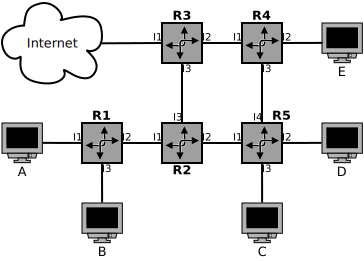
\includegraphics[width=0.50\textwidth]{img/red01.pdf}

    Donde las tablas de enrutamiento de los routers son las siguientes:

    \textbf{Router R1: }
    \begin{tabular}{|c|c|c|}
        \hline
        Destino & Máscara & Interfaz \\
        \hline
        10.0.0.224 & 255.255.255.240 & I1 \\
        \hline
        10.0.0.240 & 255.255.255.240 & I3 \\
        \hline
        0.0.0.0 & 0.0.0.0 & I2 \\
        \hline
    \end{tabular}

    \textbf{Router R2: }
    \begin{tabular}{|c|c|c|}
        \hline
        Destino & Máscara & Interfaz \\
        \hline
        10.0.0.182 & 255.255.255.254 & I2 \\
        \hline
        10.0.0.224 & 255.255.255.224 & I1 \\
        \hline
        0.0.0.0 & 0.0.0.0 & I3 \\
        \hline
    \end{tabular}

    \textbf{Router R3: }
    \begin{tabular}{|c|c|c|}
        \hline
        Destino & Máscara & Interfaz \\
        \hline
        10.0.0.180 & 255.255.255.252 & I2 \\
        \hline
        10.0.0.224 & 255.255.255.224 & I3 \\
        \hline
        0.0.0.0 & 0.0.0.0 & I1 \\
        \hline
    \end{tabular}

    \textbf{Router R4: }
    \begin{tabular}{|c|c|c|}
        \hline
        Destino & Máscara & Interfaz \\
        \hline
        10.0.0.180 & 255.255.255.254 & I2 \\
        \hline
        10.0.0.182 & 255.255.255.254 & I3 \\
        \hline
        0.0.0.0 & 0.0.0.0 & I1 \\
        \hline
    \end{tabular}

    \textbf{Router R5: }
    \begin{tabular}{|c|c|c|}
        \hline
        Destino & Máscara & Interfaz \\
        \hline
        10.0.0.183 & 255.255.255.255 & I2 \\
        \hline
        10.0.0.182 & 255.255.255.255 & I3 \\
        \hline
        0.0.0.0 & 0.0.0.0 & I1 \\
        \hline
    \end{tabular}

        \begin{enumerate}

            \item ¿Por qué routers pasará un paquete que tenga como origen el
                \emph{host C} y destino el \emph{host} con número de \emph{IP
                10.0.0.232}?

            \item ¿Por qué routers pasará un paquete que tenga como origen el
                \emph{host A} y destino el \emph{host} con número de \emph{IP
                10.0.0.197}?

        \end{enumerate}

    \item Dada la siguiente estructura de directorios:

    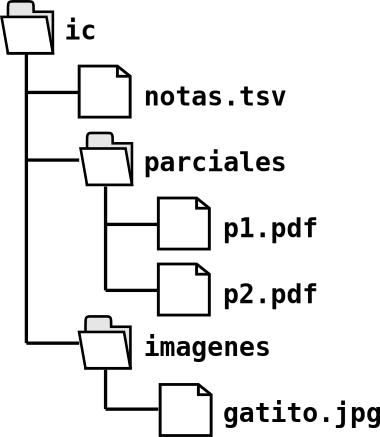
\includegraphics[width=0.50\textwidth]{img/directorios.pdf}

        \begin{enumerate}

            \item ¿Qué secuencia de comandos puede utilizar para recrearla, si
                el usuario comienza posicionado en el directorio raíz, y sin
                ningún directorio o carpeta creados?

            \item ¿Que secuencia de comandos podría utilizar para mover el
                archivo \emph{M} al directorio \emph{G}, si el usuario se
                encuentra en directorio \emph{D}?

            \item ¿Cómo puedo listar los contenidos de la carpeta \emph{B}
                sin moverme desde la carpeta \emph{J} utilizando rutas
                relativas? ¿Como se puede hacer lo mismo utilizando solo rutas
                absolutas?

        \end{enumerate}

    \item Dado el siguiente programa:

        \begin{verbatim}
     0          LD  MAX
     1          JZ  END
     2          SUB NUM
     3          ST OUT
     4          J   END
     5  END:    HLT
     6  NUM:    2
     7  MAX:    16
        \end{verbatim}

        \begin{enumerate}

            \item ¿Cuál es la salida del programa?

            \item Si se compila el programa ¿Cuál sera el contenido binario de
                las direcciones \textbf{1}, \textbf{2} y \textbf{4}?

        \end{enumerate}

    \item Dado el siguiente programa en binario:

        \begin{verbatim}
     0 01000100
     1 10001011
     2 01100100
     3 01001001
     4 11000000
     5 10001010
     6 10101001
     7 01111111
     8 00100000
     9 00000101
    10 00001010
    11 00000011
        \end{verbatim}

        ¿Cuál es la salida del programa?

    \item ¿Cual es el ciclo de compilación?

    \item ¿Por que no se puede ejecutar un archivo objeto?

\end{enumerate}

\end{document}
